% !TEX root = ../main.tex

\chapter{三角均匀部分算法}
如上文所述,光滑自由变形需将模型沿节点盒切割,并将非三角形的面片三角化。这一过程很可能产生狭长三角形或者蜕化三角形,如\autoref{subfig:clip_compare0}所示,颜色越红表示三角形质量越差。过多的此类三角形不仅会浪费计算资源,还可能带来其它数值计算方面的问题。

另一方面,沿节点盒切割只是为了保证变形结果是严格的$n$次三角贝赛尔曲面片。若略去这一步骤,算法仍能继续,只不过结果会变得不精确。考虑到在光滑自由变形中,作者采用以精度换取效率的策略,用三次的三角贝赛尔曲面来拟合n次的精确结果,也就是说光滑自由变形的结果只是精确结果的近似。因此,光滑自由变形中“沿节点盒切割以保证结果精确”这一步骤就显的可有可无了。

而且,我们通过更进一步的观察发现,在光滑自由变形中,跨多个节点盒的三角面片只要足够小,其变形后在精度上的误差,相对于在节点盒内的三角面片而言,并不会显著增加。

因此,本文尝试提出一种更好的三角形分割算法,以替换光滑自由变形中的“沿节点盒切割”这一步骤。新算法不再沿节点盒切割三角面片,而是将三角面片按以下两个要求分割成子三角形:
\begin{itemize}
    \item 所有子三角形的三边长都尽可能相等。以得到形状尽可能接近正三角形,且面积尽可能相同的子三角形。
    \item 所有子三角形的顶点均不可位于其它子三角形的边上。以避免变形后产生裂缝。
\end{itemize}

我们的新算法相比原来的沿节点盒分割的算法而言有两点优势:
\begin{itemize}
        \item 切分出来的子三角形尽可能“正”,不会产生新的狭长或蜕化的三角形。
        \item 参数$l$使得用户可以控制产生的子三角形的大小。
\end{itemize}


\section{算法实现}
首先我们先定义一些符号以方便描述算法实现。$l$,$t$为算法的输入,$l$表示子三角形边长的期望值,算法分割产生的子三角形的三边的长度需尽可能接近$l$。$t$表示待分割的三角面片。$\{e_i\}^{2}_{i=0}$为$t$的三条边。$\{len_i\}^{2}_{i=0}$代表三边的边长。$t$的每条边会被均匀分成$\lceil len_i/l \rceil$段。$p_{ij}$表示三角形第i条边的第j个分割点。

算法流程:
\begin{enumerate}
    \item 找出三角面片最小的内角$\alpha$,不妨假定角$\alpha$的两条边为$e_0$, $e_1$。
    \item 将$e_0$、$e_1$分别均匀分成$\lceil len_0/l \rceil$、$\lceil len_0/l \rceil$段,产生的切割点的有序集合\footnote{切割点包括边的首尾端点}为$\{p_{0j}\}^{\lceil len_0/l \rceil}_{j=0}$、$\{p_{1j}\}^{\lceil len_1/l \rceil}_{j=0}$,且$j$沿角$\alpha$的顶点至另一端点方向依次增长。分割点如\autoref{subfig:clip1}所示。
    \item 将子三角形$p_{00}p_{01}p_{11}$分割下来,如\autoref{subfig:clip2}所示。
    \item 剩下的部分是一个类似于梯形的四边形,如\autoref{subfig:clip2}中红色部分所示。如果$\lceil len_0/l \rceil == \lceil len_1/l \rceil$,我们依次将四边形$\{p_{0j}p_{1j}p_{1(j+1)}p_{0(j+1)}\}^{\lceil len_0/l \rceil - 1}_{j=0}$分割成子三角形,如\autoref{subfig:clip6}、\autoref{subfig:clip9}所示,直到将所有四边形均分割完毕,然后直接跳转到步骤\ref{CVT};否则\footnote{$\lceil len_0/l \rceil \ne \lceil len_1/l \rceil$},我们依次将四边形$\{p_{0j}p_{1j}p_{1(j+1)}p_{0(j+1)}\}^{min(\lceil len_0/l \rceil, \lceil len_1/l \rceil) - 2}_{j=0}$分割成子三角形,剩余部分如\autoref{subfig:clip16}所示。\label{recursion}
    \item \autoref{subfig:clip16}中剩余部分若逆时针旋转90度,我们可以发现剩余部分和\autoref{subfig:clip3}类似。所以我们递归的进行步骤\ref{recursion},直到三角形分割完毕。\label{recursion2}
    \item 对分割结果进行5次CVT优化,使子三角形边长更加接近$l$。\label{CVT}
\end{enumerate}

在步骤\ref{recursion2}中,递归到最后阶段,可能会出现步骤\ref{recursion}处理不了的特殊情况。但是特殊情况的类型不会很多,所以我们为每一种特殊情况指定了对应的分割方案。

\begin{figure}[htbp]
	\centering
	\begin{subfigure}[b]{.32\textwidth}
		\centering
		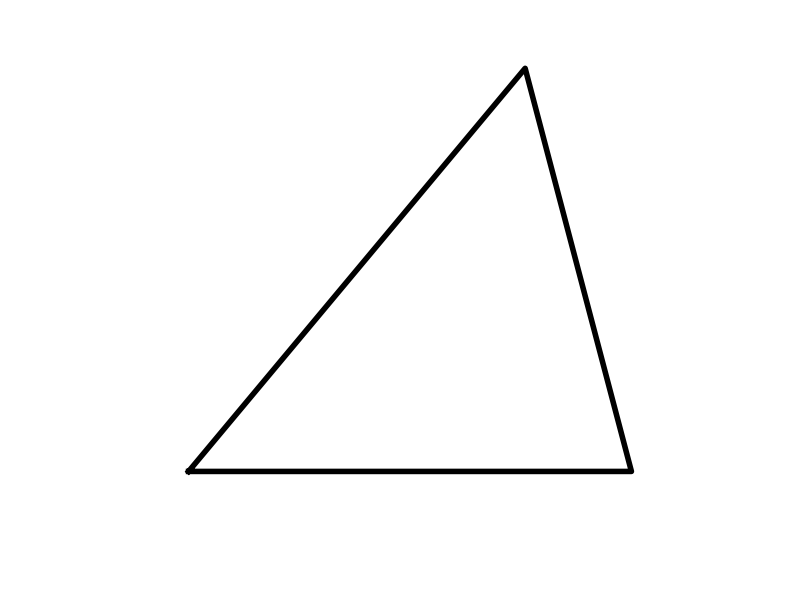
\includegraphics[width = \textwidth]{clip_figure0.png}
		\caption{初始三角面片}\label{subfig:clip0}
	\end{subfigure}
	\begin{subfigure}[b]{.32\textwidth}
		\centering
		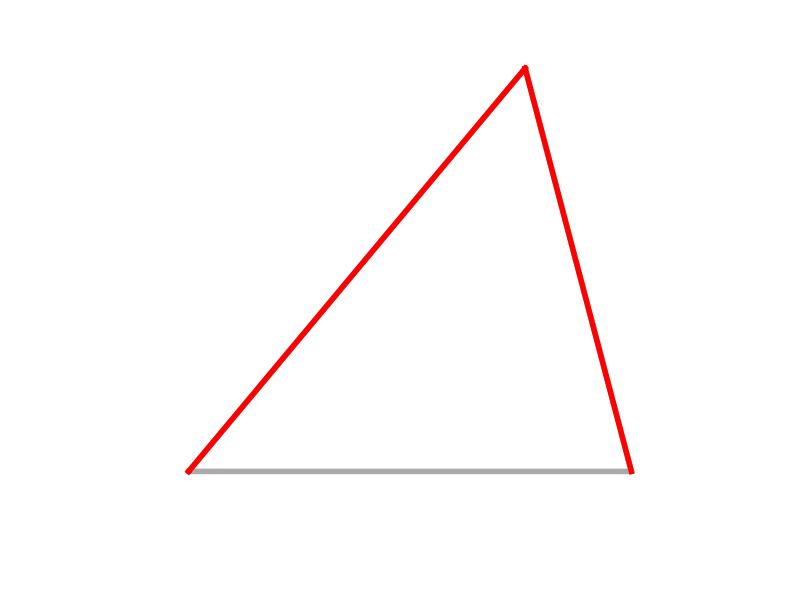
\includegraphics[width = \textwidth]{clip_figure1.png}
		\caption{初始三角面片}\label{subfig:clip1}
	\end{subfigure}
	\begin{subfigure}[b]{.32\textwidth}
		\centering
		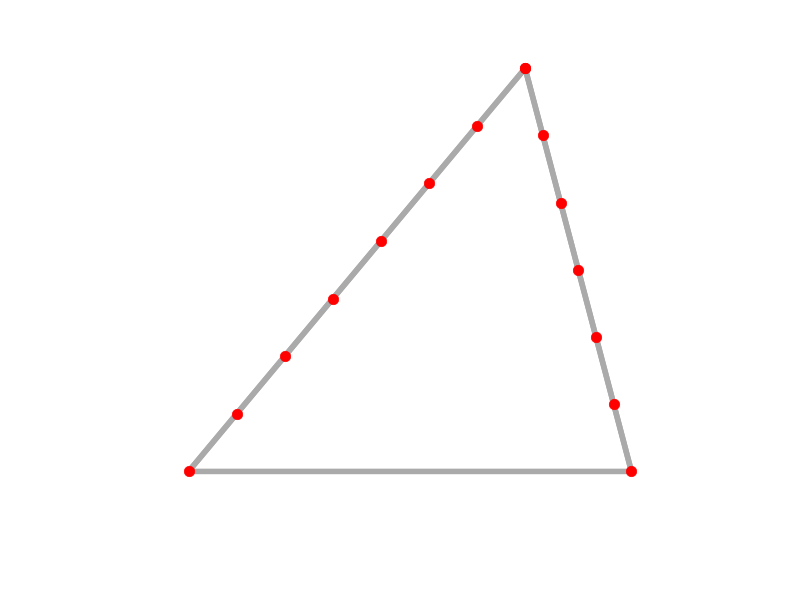
\includegraphics[width = \textwidth]{clip_figure2.png}
		\caption{分割最小角$\alpha$的两条边}\label{subfig:clip2}
	\end{subfigure}

	\begin{subfigure}[b]{.32\textwidth}
		\centering
		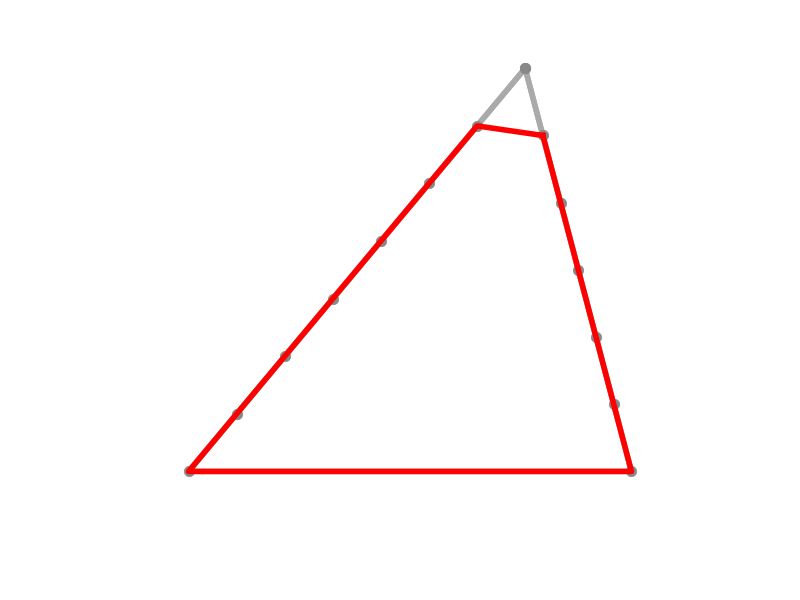
\includegraphics[width = \textwidth]{clip_figure3.png}
		\caption{切割第一个子三角形}\label{subfig:clip3}
	\end{subfigure}
	\begin{subfigure}[b]{.32\textwidth}
		\centering
		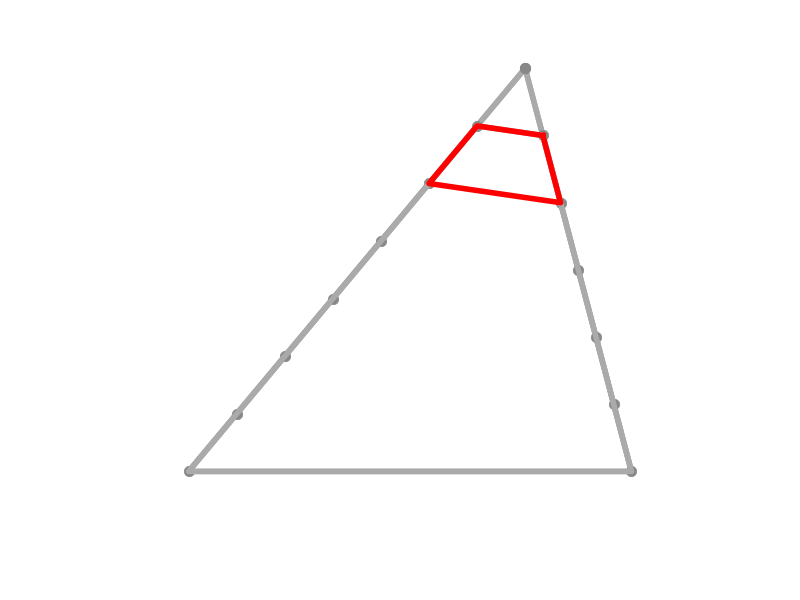
\includegraphics[width = \textwidth]{clip_figure4.png}
		\caption{第一个待分割层}\label{subfig:clip4}
	\end{subfigure}
	\begin{subfigure}[b]{.32\textwidth}
		\centering
		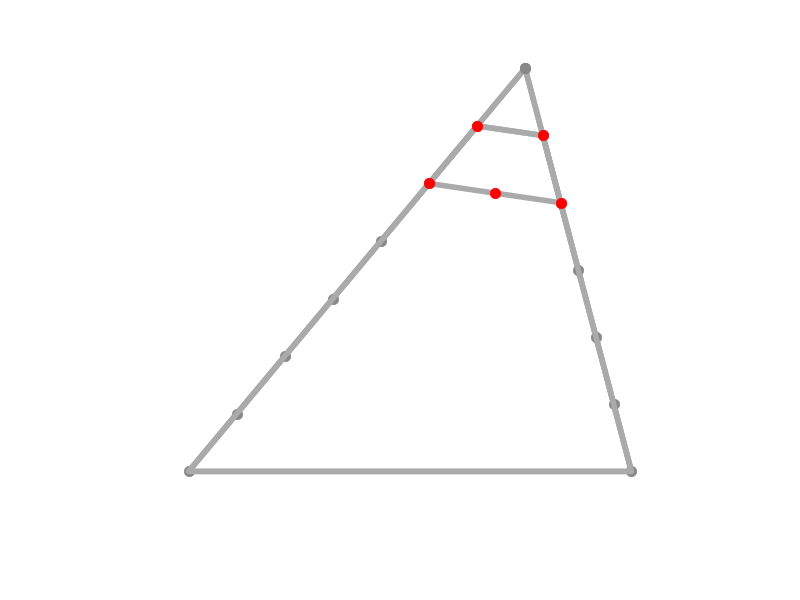
\includegraphics[width = \textwidth]{clip_figure5.png}
		\caption{分割待分割层的上下底边}\label{subfig:clip5}
	\end{subfigure}

	\begin{subfigure}[b]{.32\textwidth}
		\centering
		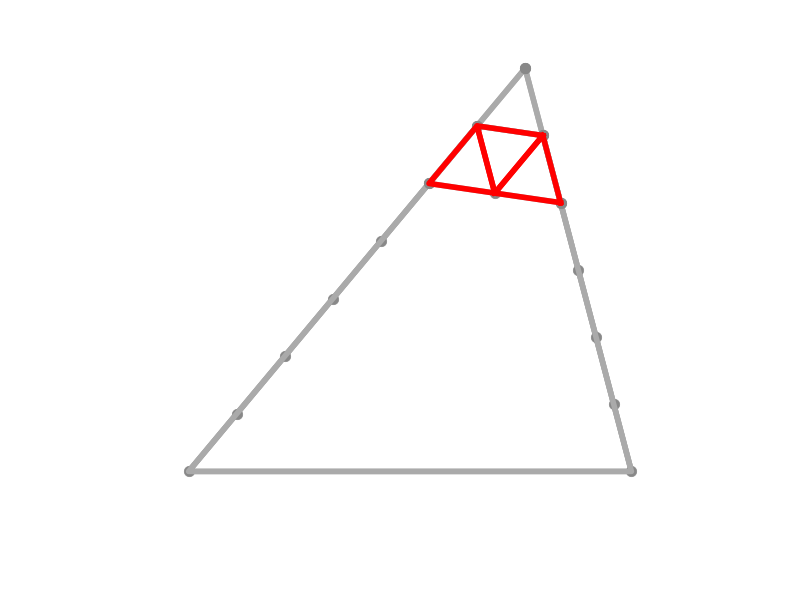
\includegraphics[width = \textwidth]{clip_figure6.png}
		\caption{分割待侵害层的上下底边}\label{subfig:clip6}
	\end{subfigure}
	\begin{subfigure}[b]{.32\textwidth}
		\centering
		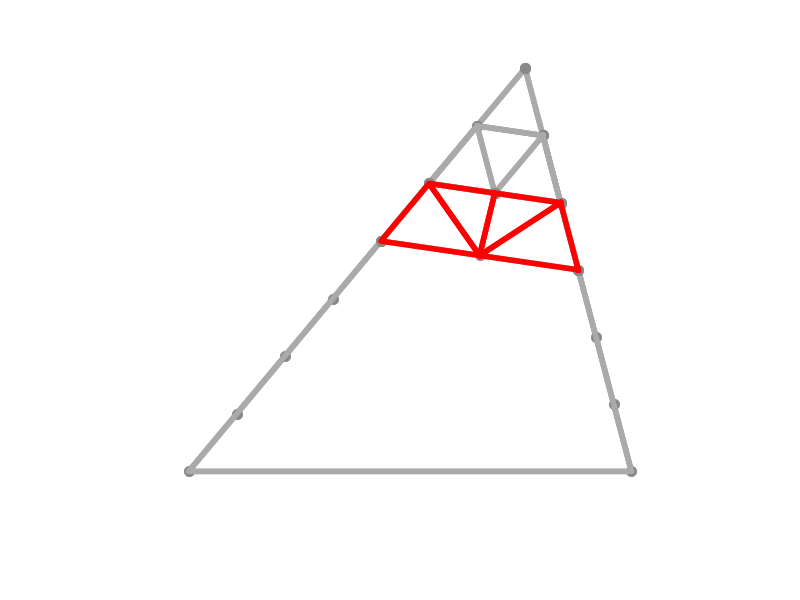
\includegraphics[width = \textwidth]{clip_figure9.png}
		\caption{分割待侵害层的上下底边}\label{subfig:clip9}
	\end{subfigure}
	\begin{subfigure}[b]{.32\textwidth}
		\centering
		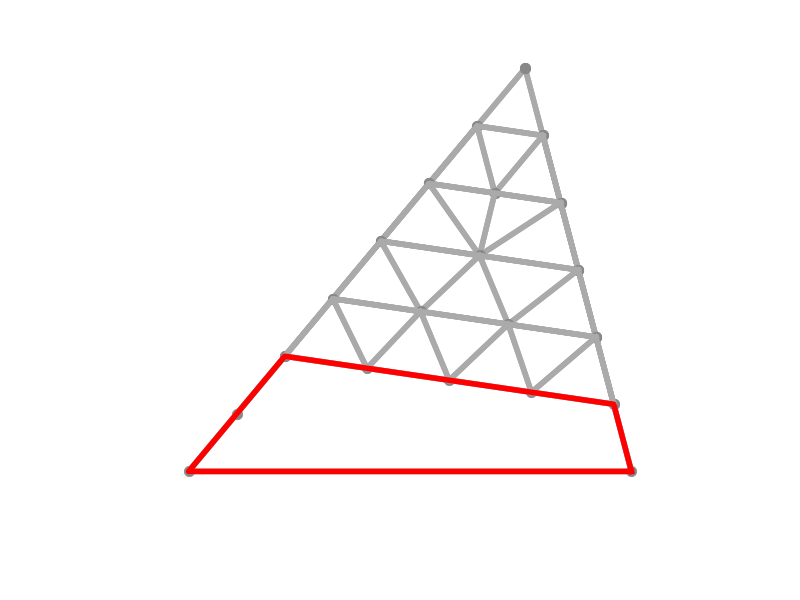
\includegraphics[width = \textwidth]{clip_figure16.png}
		\caption{继续侵害红色部分}\label{subfig:clip16}
	\end{subfigure}

	\begin{subfigure}[b]{.32\textwidth}
		\centering
		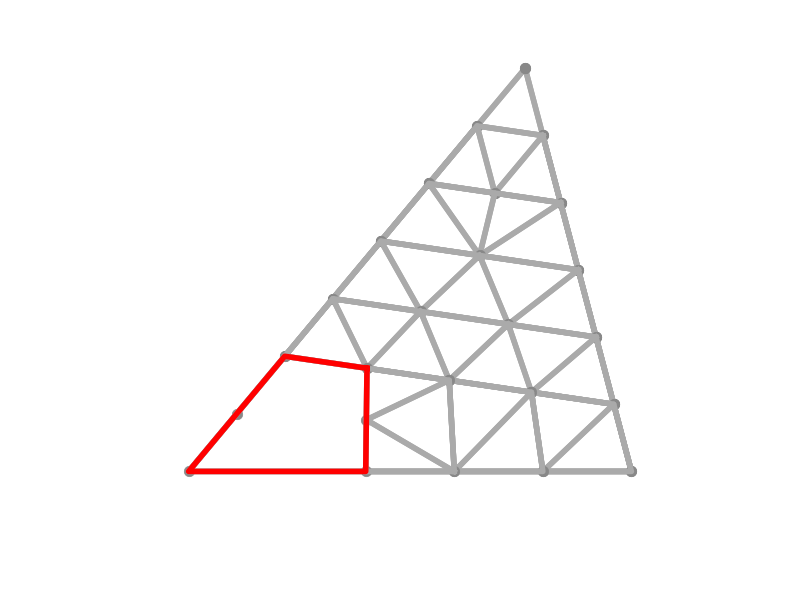
\includegraphics[width = \textwidth]{clip_figure26.png}
		\caption{对特殊情况进行处理}\label{subfig:clip26}
	\end{subfigure}
	\begin{subfigure}[b]{.32\textwidth}
		\centering
		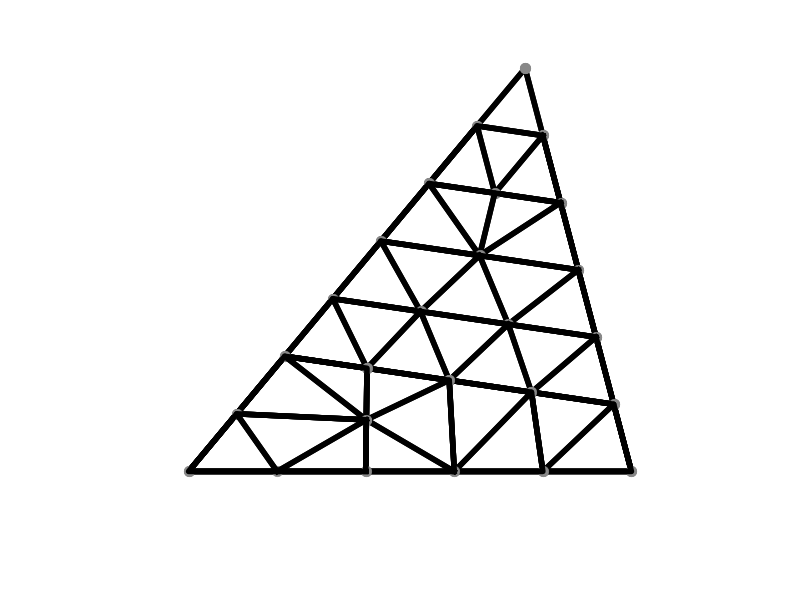
\includegraphics[width = \textwidth]{clip_figure33.png}
		\caption{分割结果}\label{subfig:clip33}
	\end{subfigure}
	\begin{subfigure}[b]{.32\textwidth}
		\centering
		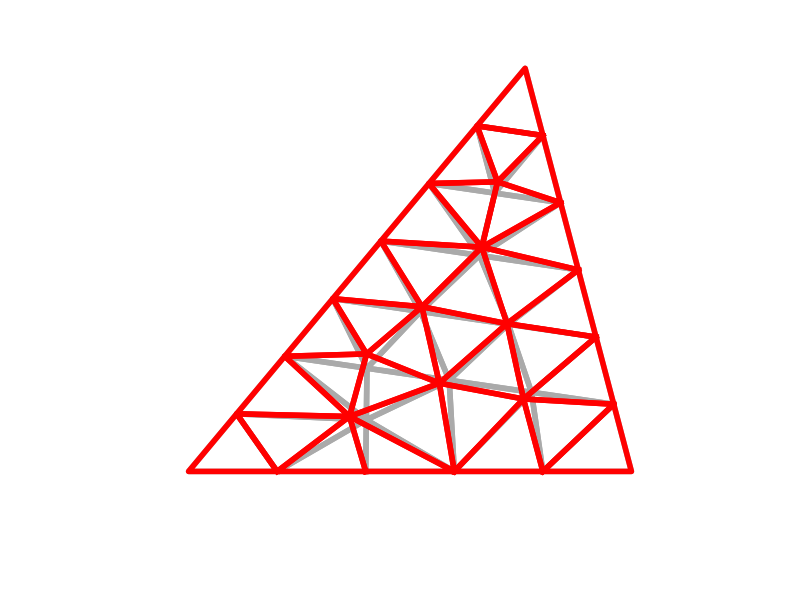
\includegraphics[width = \textwidth]{clip_figure34.png}
		\caption{对结果进行CVT优化}\label{subfig:clip34}
	\end{subfigure}
	\caption{均匀三角剖分算法}\label{fig:clip}
\end{figure}

CVT\cite{du1999}优化可以使分割更加均匀。且该过程可以迭代进行,使分割结果越来越均匀。\autoref{fig:CVT}展示了迭代过程,红色是优化之后的结果,灰色的是优化之前的。我们可以发现,第5次及之后的迭代收益不大。所以我们最终对结果进行5次CVT迭代优化。

\begin{figure}[htbp]
	\centering
	\begin{subfigure}[b]{.49\textwidth}
		\centering
		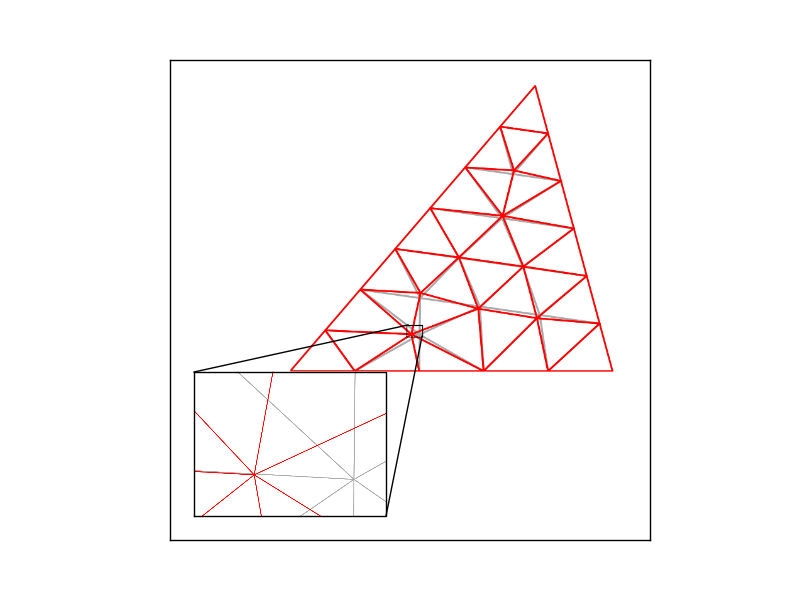
\includegraphics[width = \textwidth]{cvt_for_paper0.png}
		\caption{第1次CVT优化}
	\end{subfigure}
	\begin{subfigure}[b]{.49\textwidth}
		\centering
		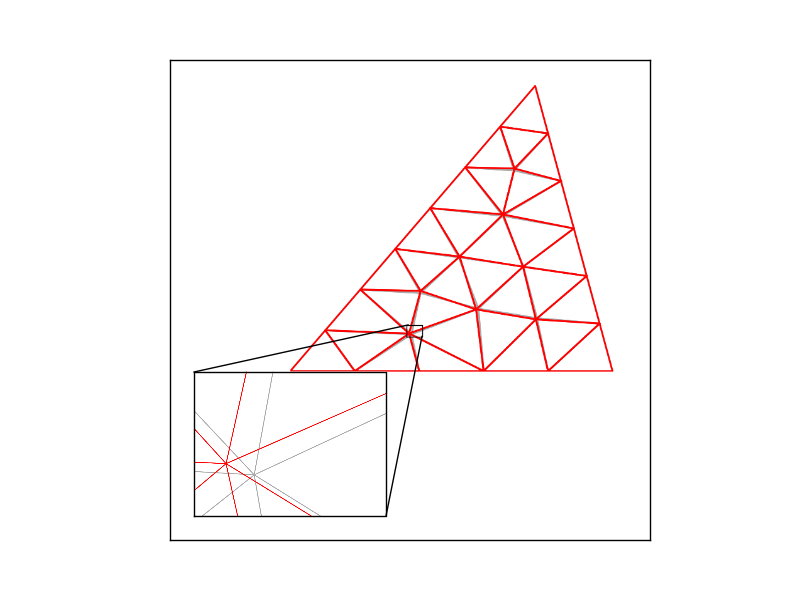
\includegraphics[width = \textwidth]{cvt_for_paper1.png}
		\caption{第2次CVT优化}
	\end{subfigure}

	\begin{subfigure}[b]{.49\textwidth}
		\centering
		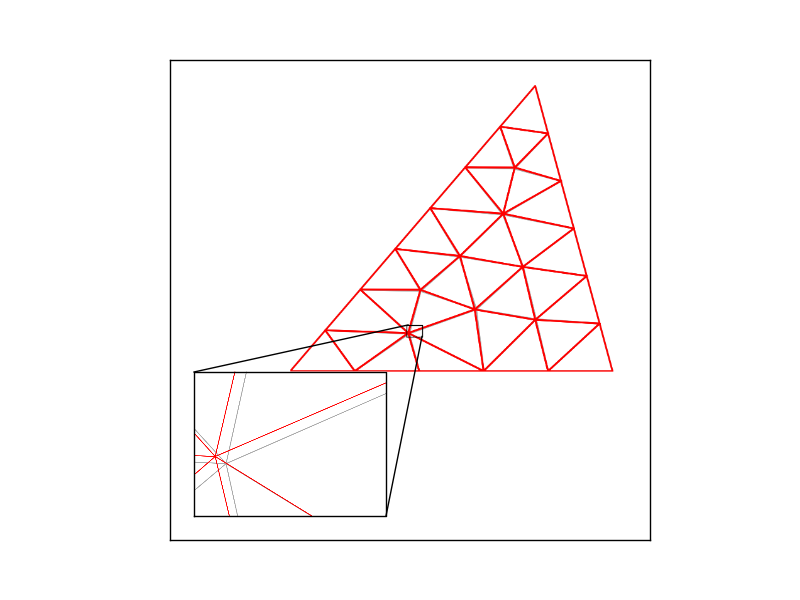
\includegraphics[width = \textwidth]{cvt_for_paper2.png}
		\caption{第3次CVT优化}
	\end{subfigure}
	\begin{subfigure}[b]{.49\textwidth}
		\centering
		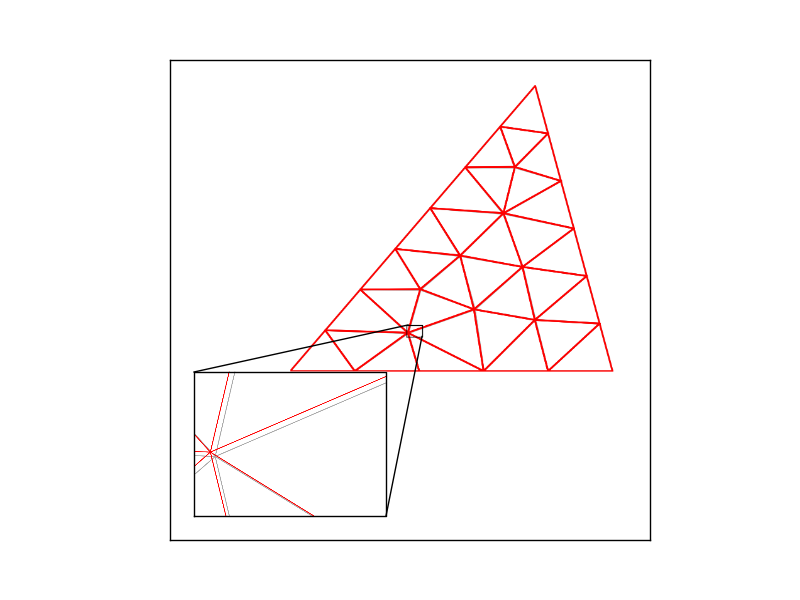
\includegraphics[width = \textwidth]{cvt_for_paper3.png}
		\caption{第4次CVT优化}
	\end{subfigure}

	\begin{subfigure}[b]{.49\textwidth}
		\centering
		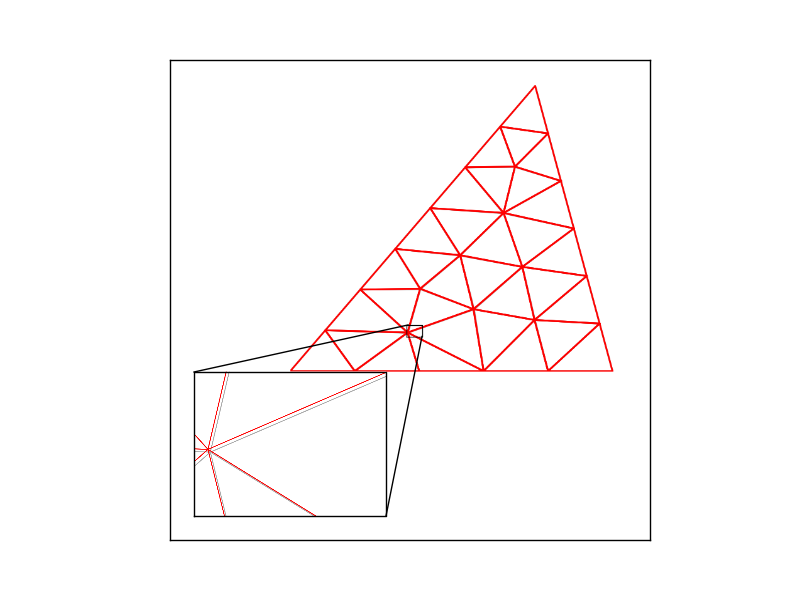
\includegraphics[width = \textwidth]{cvt_for_paper4.png}
		\caption{第5次CVT优化}
	\end{subfigure}
	\begin{subfigure}[b]{.49\textwidth}
		\centering
		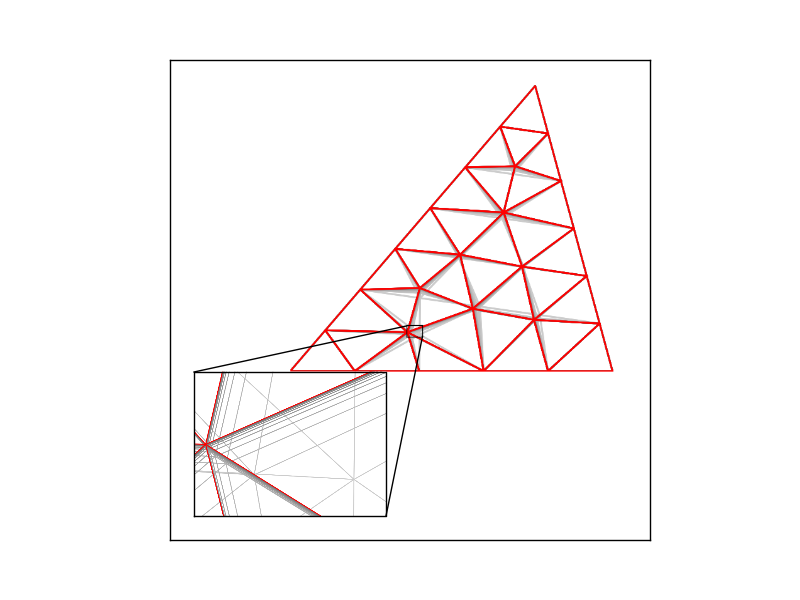
\includegraphics[width = \textwidth]{cvt_for_paper5.png}
		\caption{1~10次CVT优化}
	\end{subfigure}
    \caption{CVT优化结果} \label{fig:CVT}
\end{figure}

\section{关于$l$的讨论}
前文提到的$l$是一个很关键的参数,$l$不仅会影响算法效率、子三角形的质量\footnote{这里的质量表示接近正三角形的程度}、还能影响变形结果的精度。但是,$l$并不是影响这些的直接因素,对子三角形的质量和算法效率产生直接影响的是子三角形的数目,而对变形结果的精度产生直接影响的是子三角形的平均面积。$l$则通过改变子三角形数目或平均面积,间接地对算法效率、子三角形的质量、变形结果的精度产生影响。

定性的来说$l$越小,子三角形数目越多,面积越小,同时子三角形的质量越高,变形结果的误差越小,但算法的计算代价越高。为了进一步明确$l$对算法的影响,我们进行了一系列实验以定量的分析$l$。

实验选用了立方体模型,有12个面片,且模型被归一化到$[-1, 1]^3$。之所以选择由大三角面片组成的模型,是为了让三角面片随$l$变化切割出不同大小的子三角形。\autoref{fig:l-number}显示了$l$与子三角形数量的关系,蓝色表示以立方体为模型进行切割,立方体原始的三角面片平均面积为2.0,绿色表示以兔子玩偶为模型进行切割,兔子玩偶原始的三角面片平均面积为0.0007。从中我们可以发现兔子玩偶模型原始三角片面过小,当$l$大于某个值的时候,其不再被切割,子三角形的数目也保持不变,这样不利于我们探索$l$在对变形算法产生的影响。而立方体由于原始三角面片较大,能随$l$变大切割出不同数目的子三角形。可以帮助我们更好的研究$l$对算法的影响。

变形空间的次数是$3\times3\times3$,控制顶点个数是$5\times5\times5$。实验的自变量是$l$,由$0.1$增长到$2\sqrt{3}$\footnote{$2\sqrt{3}$为变形空间对角线长度}。因变量是算法效率、子三角形的质量、变形结果的精度。以下是实验结果。

%兔子模型的平均三角形面积为总表面积/三角形数目
%5.880918 / 8400 = 0.0007001092857142858
\begin{figure}[htbp]
	\centering
	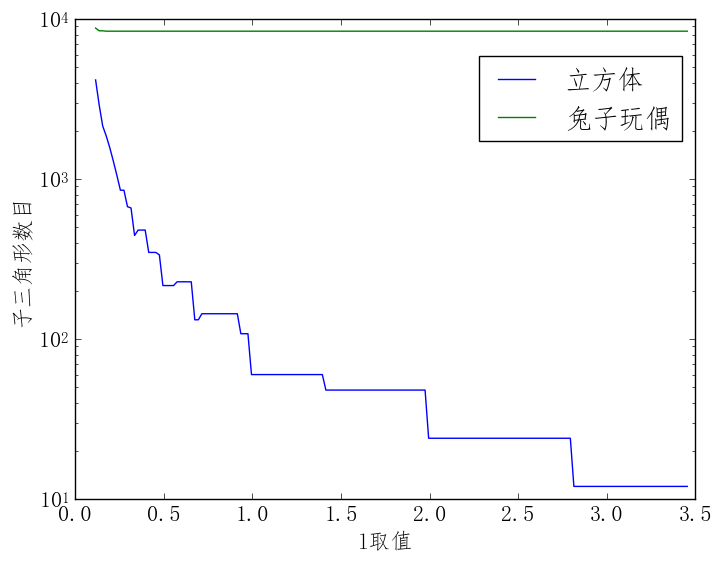
\includegraphics[width = 0.8\textwidth]{l-number.png}
	\caption{$l$取值-子三角形数目关系图}\label{fig:l-number}
\end{figure}

\subsection{算法效率}
虽然自变量是$l$,但从\autoref{fig:l-number}可以看出不同的$l$可以对应相同的子三角形数目


\begin{figure}[htbp]
	\centering
	\begin{subfigure}[b]{.45\textwidth}
	    \centering
	    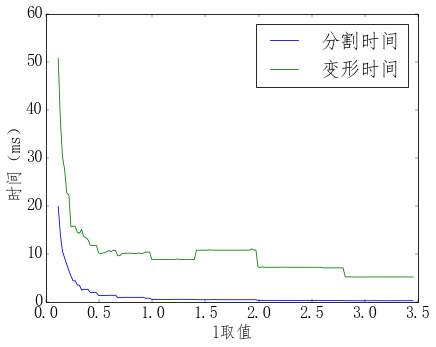
\includegraphics[width =\textwidth]{l-time0.png}
	    \caption{$l$取值-算法运行时间关系图}\label{fig:l-time0}
	\end{subfigure}
	\begin{subfigure}[b]{.45\textwidth}
	    \centering
	    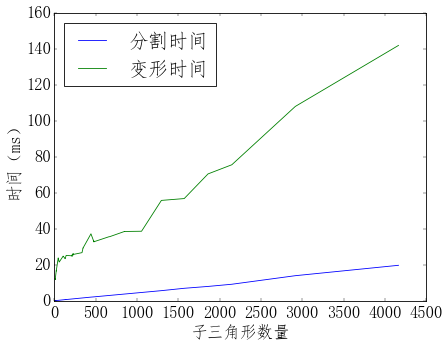
\includegraphics[width =\textwidth]{l-time1.png}
	    \caption{三角形数目-算法运行时间关系图}\label{fig:l-time1}
	\end{subfigure}
	\caption{$l$取值-算法效率}\label{fig:l-time0}
\end{figure}

\subsection{子三角形质量}
有很多指标都可以衡量三角形质量\cite{pebay2003},我们选取了其中计算量较少的一个$q(t)=r_t/max(\{e_i\}^{2}_{i=0})$,即三角形外接圆的半径除以其最长边。该指标的取值范围是$(0, \frac{\sqrt{3}}{2}]$,当三角形$t$为正三角形时,$q(t)$取到最大值$\frac{\sqrt{3}}{2}$;三角形$t$越狭长,$q(t)$的值越接近0。为了更直观的用该指标表示三角形质量,我们修改将$q(t)$修改为$q(t)=r_t/max(\{e_i\}^{2}_{i=0})*2\sqrt{3}$,使其取值范围为$(0, 1]$。\autoref{fig:triangle_quality_compare}可视化了两种三角形分割方法产生的三角形的质量,可见本文方法产生的三角形质量要好很多。

\begin{figure}[htbp]
	\centering
	\begin{subfigure}[b]{.4\textwidth}
		\centering
		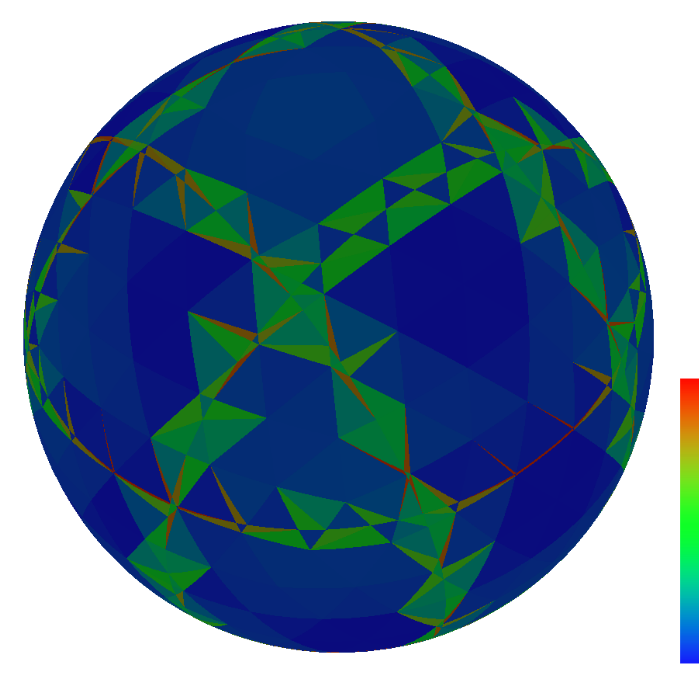
\includegraphics[width = \textwidth]{clip_compare0.png}
		\caption{沿节点盒切割}\label{subfig:clip_compare0}
	\end{subfigure}%
	\begin{subfigure}[b]{.4\textwidth}
		\centering
		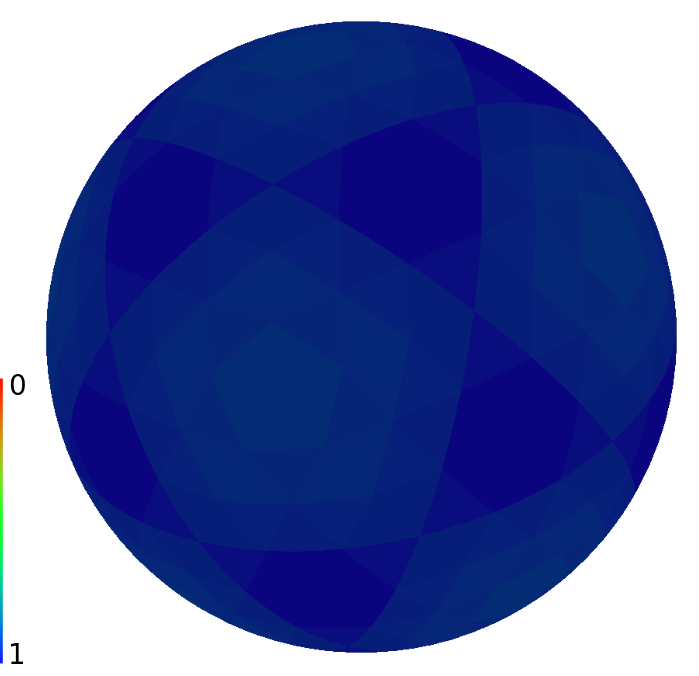
\includegraphics[width = \textwidth]{clip_compare1.png}
		\caption{本文方法}\label{subfig:clip_compare1}
	\end{subfigure}
	\caption{两种切割算法产生的子三角形的质量对比}\label{fig:triangle_quality_compare}
\end{figure}

对于不同的$l$对三角形质量的影响如所示\textcolor{red}{需另外作图},可见$l$越小,三角形质量越高\textcolor{red}{添加更加详细的结论}。

\subsection{变形结果精度}
如前方所述,三角形面积过大,误差就会增加;三角形面积过小,误差会相应减小,但同时三角形数目会增加,造成浪费计算的资源。我们需要找出合适大小的$l$,使结果精度和效率有一个较好的平衡。为此我们用不同的$l$分割了各种不同类型的模型,得到如\autoref{fig:l}所示的结果。

\begin{figure}[htbp]
	\centering
	\begin{subfigure}[b]{.2\textwidth}
		\centering
		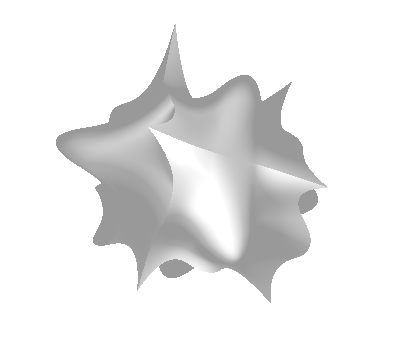
\includegraphics[width = \textwidth]{ln_cube_e.png}
		\label{subfig:ln_cube_e}
	\end{subfigure}
	\begin{subfigure}[b]{.35\textwidth}
		\centering
		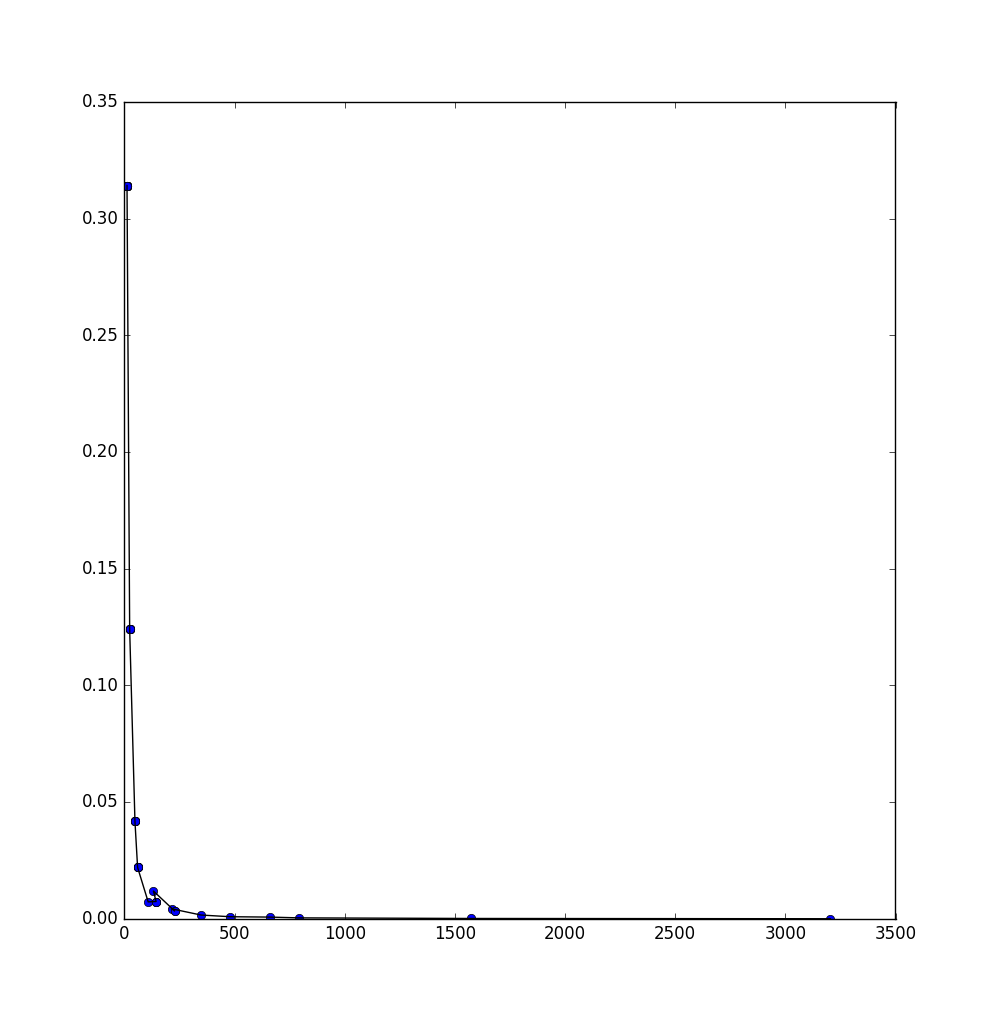
\includegraphics[width = \textwidth]{ln_cube.png}
		\label{subfig:ln_cube}
	\end{subfigure}
    \quad
	\begin{subfigure}[b]{.35\textwidth}
		\centering
		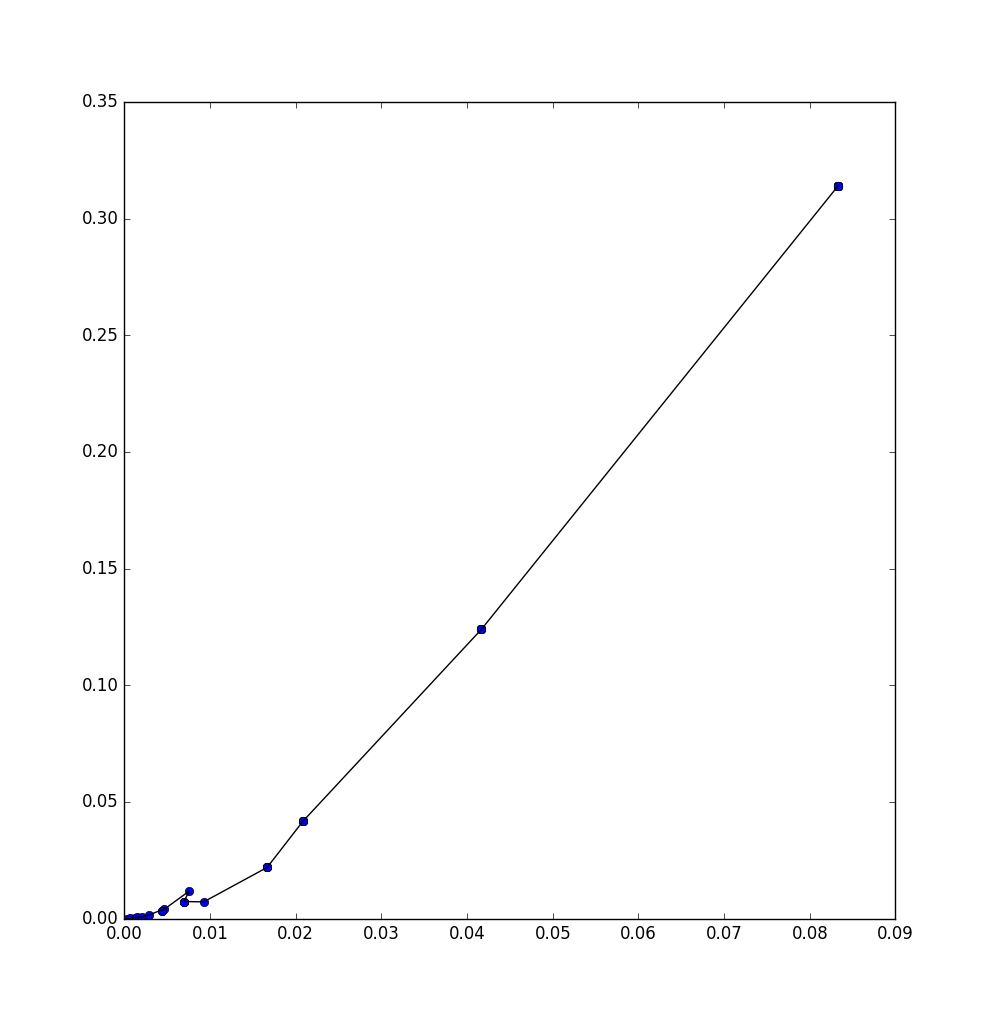
\includegraphics[width = \textwidth]{ln_r_cube.png}
		\label{subfig:ln_r_cube}
	\end{subfigure}

	\begin{subfigure}[b]{.2\textwidth}
		\centering
		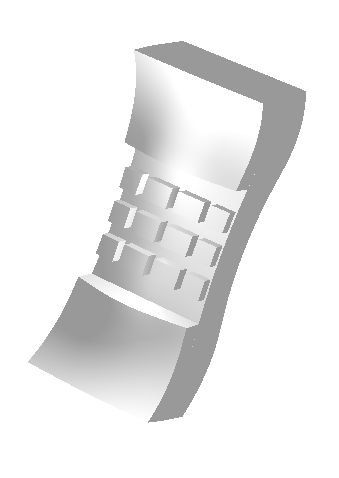
\includegraphics[width = \textwidth]{ln_mobile_e.png}
		\label{subfig:ln_mobile_e}
	\end{subfigure}
    \quad
	\begin{subfigure}[b]{.35\textwidth}
		\centering
		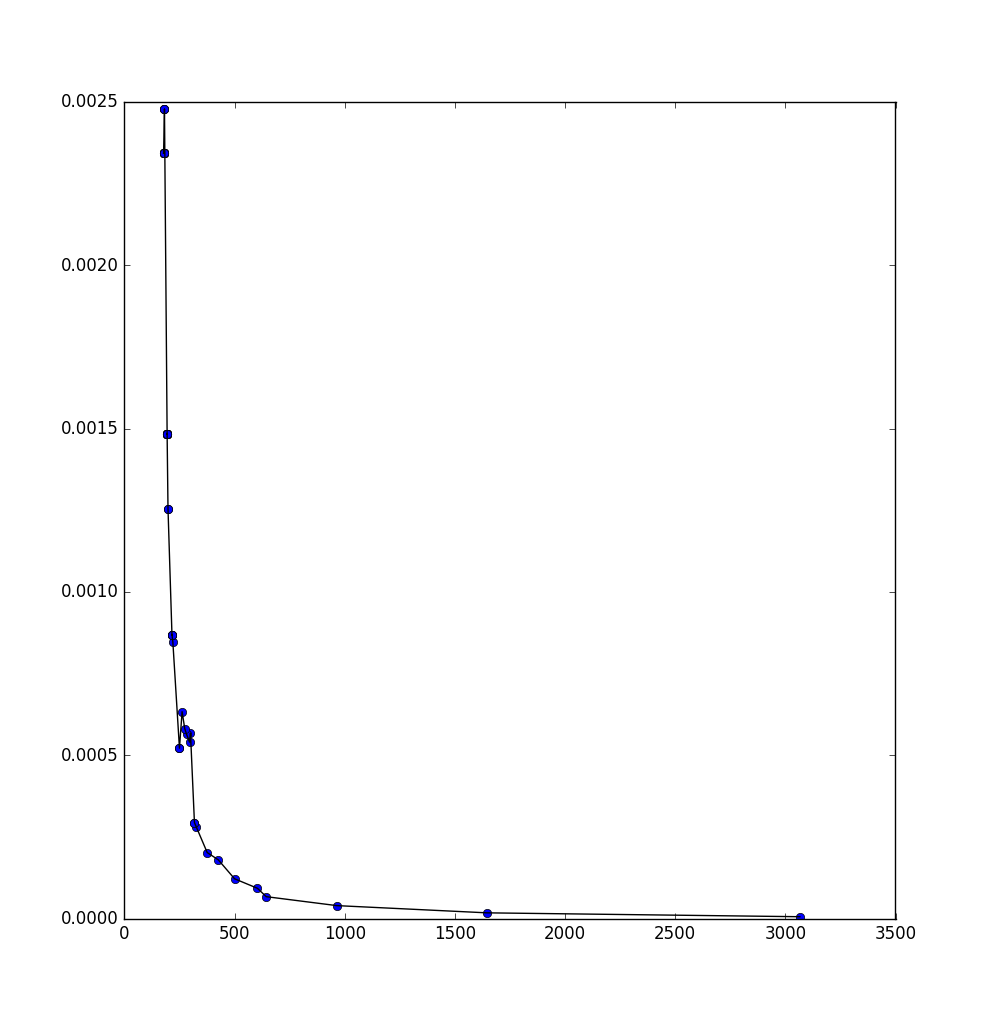
\includegraphics[width = \textwidth]{ln_mobile.png}
		\label{subfig:ln_mobile}
	\end{subfigure}
    \quad
	\begin{subfigure}[b]{.35\textwidth}
		\centering
		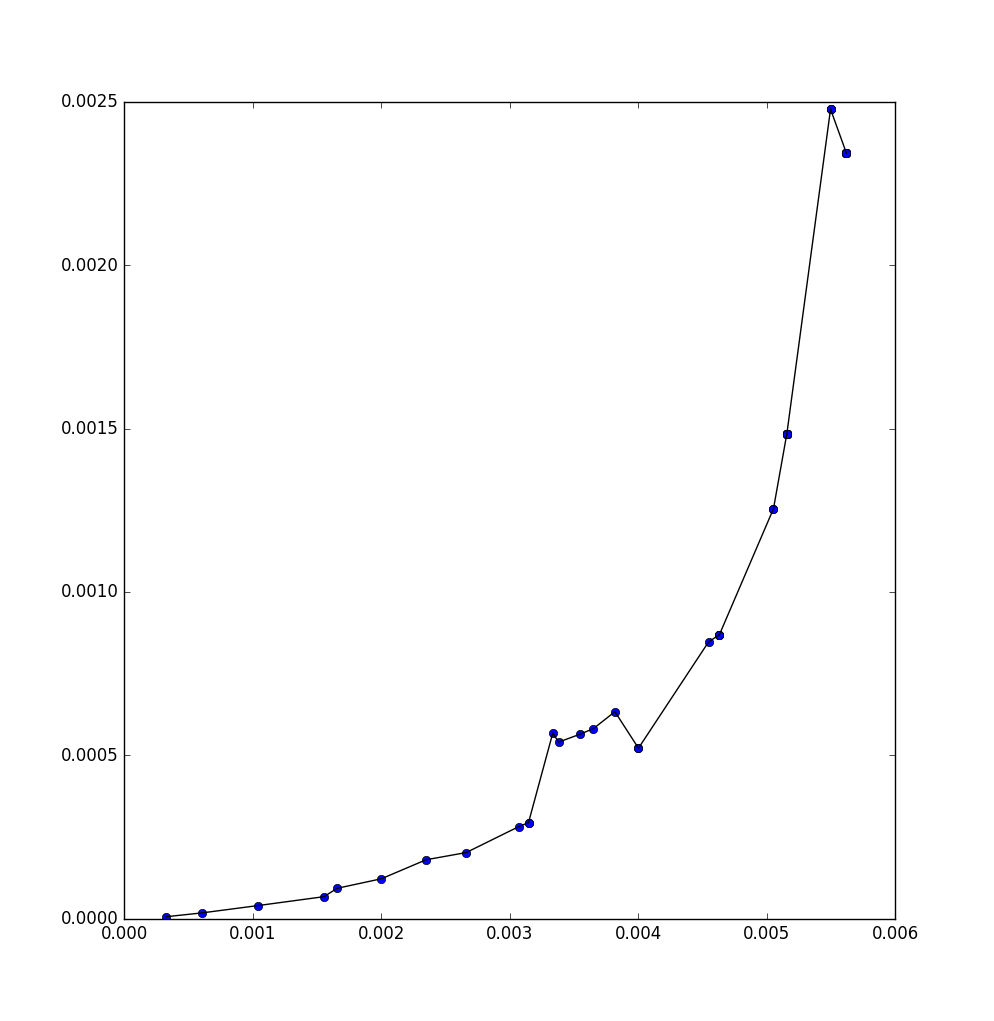
\includegraphics[width = \textwidth]{ln_r_mobile.png}
		\label{subfig:ln_r_mobile}
	\end{subfigure}

	\begin{subfigure}[b]{.2\textwidth}
		\centering
		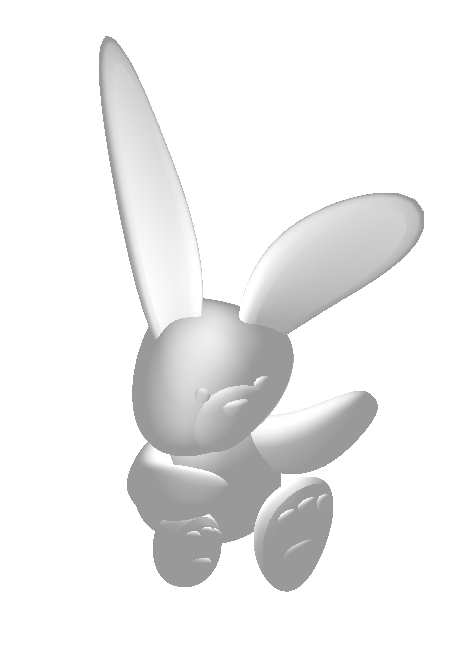
\includegraphics[width = \textwidth]{ln_bear_e.png}
		\label{subfig:ln_bear_e}
	\end{subfigure}
    \quad
	\begin{subfigure}[b]{.35\textwidth}
		\centering
		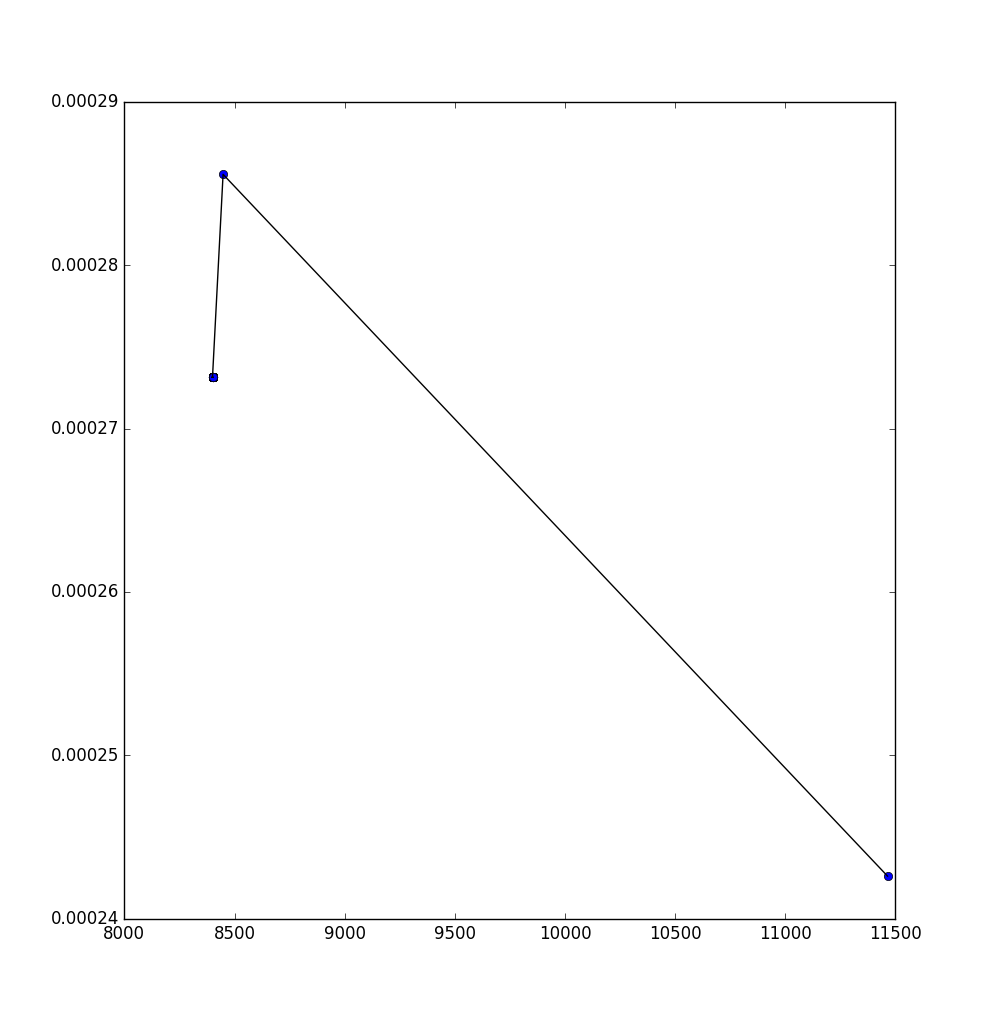
\includegraphics[width = \textwidth]{ln_bear.png}
		\label{subfig:ln_bear}
	\end{subfigure}
    \quad
	\begin{subfigure}[b]{.35\textwidth}
		\centering
		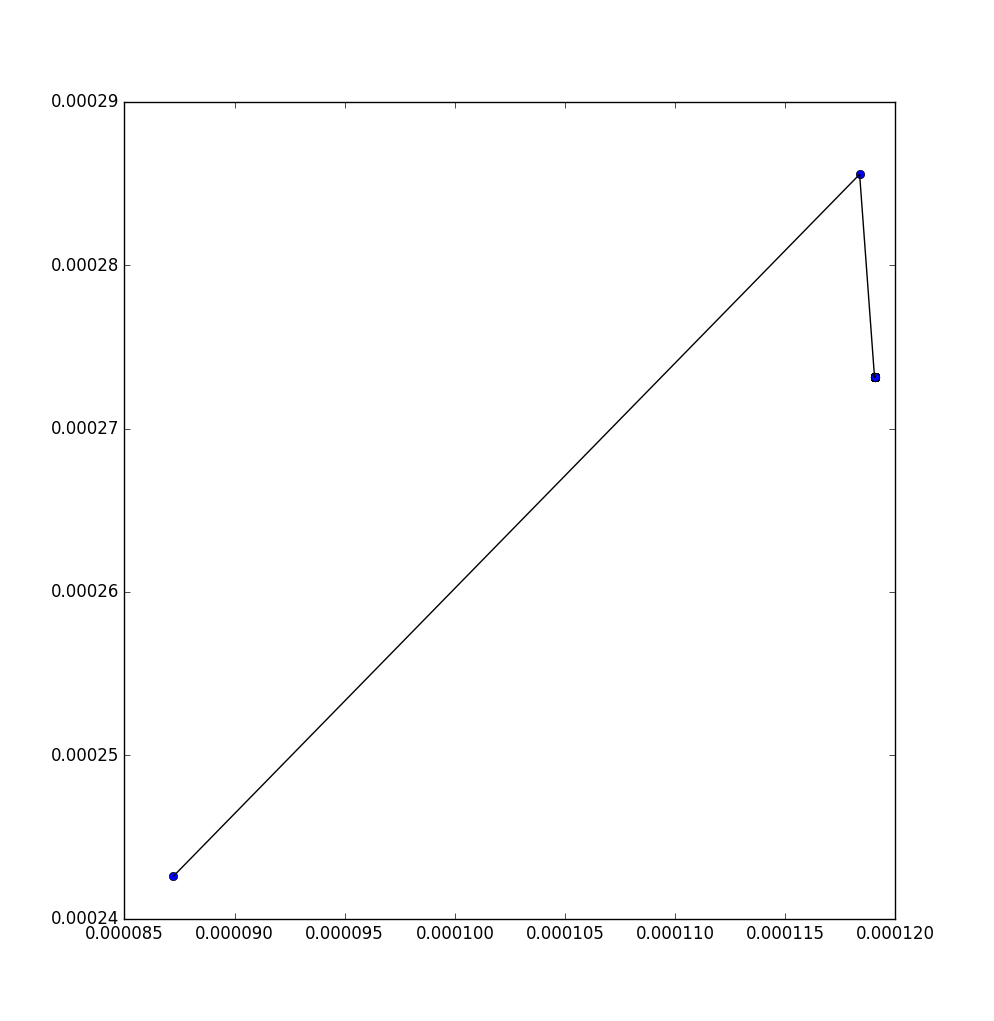
\includegraphics[width = \textwidth]{ln_r_bear.png}
		\label{subfig:ln_r_bear}
	\end{subfigure}

	\caption{三角形数目对变形结果的影响}\label{fig:l}
\end{figure}

\section{demo}
以下是一个测试用的列表环境,内容不要在意。\footnote{正文中中脚注命令测试,长脚注情况:这包括如下事实:“未经本人同意,监听、录制或转播私人性质的谈话或秘密谈话;未经本人同意,拍摄、录制或转播个人在私人场所的形象”}

\begin{enumerate}
	\item 第一级列表\label{itm:11}
	\begin{enumerate}
		\item 第二级列表\label{itm:12}
	\end{enumerate}
\end{enumerate}

\begin{itemize}
	\item 第一级列表
	\begin{itemize}
		\item 第二级列表
	\end{itemize}
\end{itemize}

\section{浮动体测试}
\subsection{插图测试}
如\autoref{fig:first_image_tset}是对此模版的第一张插图测试。

\begin{figure}[htbp]
	\centering
	
\includegraphics[width = 0.5\linewidth]{Chapter1.png}
	\caption{第一张插图测试}\label{fig:first_image_tset}
\end{figure}

\subsection{表格测试}

\subsubsection{array宏包tabular表格环境测试}
如\autoref{tab:first_table_test}是对array宏包的tabular表格环境测试。
\begin{table}[htbp]
	\centering
	\caption{这是一个用tabular环境的测试用的表格}\label{tab:first_table_test}
    \begin{tabular}{lrr}
    \toprule
    \textbf{行星}     & \textbf{赤道半径}km & \textbf{公转周期}d \\
    \midrule
    水星     & 2.439  & 87.9 \\
    金星     & 6.1    & 224.682 \\
    地球     & 6378.14 & 365.24 \\
    \bottomrule
    \end{tabular}%
\end{table}

\subsubsection{tabu宏包表格环境测试}
如\autoref{tab:tabu_test_1}是对tabu宏包的tabu表格环境测试。在这里表格命令与\autoref{tab:first_table_test}的命令相同,只是tabular环境改成了tabu环境。
\begin{table}[htbp]
	\centering
	\caption{这是一个用tabu环境的测试用的表格}\label{tab:tabu_test_1}
    \begin{tabu}{lrr}
    \toprule
    \textbf{行星}     & \textbf{赤道半径}km & \textbf{公转周期}d \\
    \midrule
    水星     & 2.439  & 87.9 \\
    金星     & 6.1    & 224.682 \\
    地球     & 6378.14 & 365.24 \\
    \bottomrule
    \end{tabu}%
\end{table}

\autoref{tab:tabu_test_2}对tabu to表格的x列模式进行测试。在表格导言区中设置为X[1]X[2]X[2],表示这三列表格的列宽比值为1:2:2,总的表格宽度由tabu to环境设置,这里设置为0.6\textbackslash linewidth。相比于tabular环境,tabu环境的列宽设置方便许多。
\begin{table}[htbp]
	\centering
	\caption{tabu环境测试表格---X列模式}\label{tab:tabu_test_2}
    \begin{tabu} to 0.6\linewidth{X[1]X[2]X[2]}
    \toprule
    \textbf{行星}     & \textbf{赤道半径}km & \textbf{公转周期}d \\
    \midrule
    水星     & 2.439  & 87.9 \\
    金星     & 6.1    & 224.682 \\
    地球     & 6378.14 & 365.24 \\
    \bottomrule
    \end{tabu}%
\end{table}

特别需要注意的是,longtabu是基于longtable宏包开发的,所以在zjuthesis.cls文件中已经插入了longtable宏包。longtable环境的所有功能都可以在longtabu中使用,如\textbackslash endhead,\textbackslash endfirsthead,\textbackslash endfoot,\textbackslash endlastfoot,和\textbackslash caption等。具体用法请参见longtable和tabu宏包的相应文档。
\begin{longtabu}{lccc}
\caption{材料弹性模量及泊松比}\label{tab:tabu_test_3}\\
\toprule
名  称   & 弹性模量E/Gpa & 切变模量G/Gpa & 泊松比$\mu$ \\
\midrule%
\endfirsthead
\caption{材料弹性模量及泊松比(续)}\\
\toprule
名  称   & 弹性模量E/Gpa & 切变模量G/Gpa & 泊松比$\mu$ \\
\midrule%
\endhead
\bottomrule%
\endfoot
镍铬钢、合金钢 & 206    & 79.38  & 0.3 \\
碳 钢    &  196~206 & 79     & 0.3 \\
\end{longtabu}%

\subsection{子图}

如\autoref{fig:subfig_test1}是有两张子图的模式,对子图进行交叉引用,如\autoref{subfig:1a}和\autoref{subfig:1b}。

\begin{figure}[htbp]
	\centering
	\begin{subfigure}[b]{.4\textwidth}
		\centering
		
\includegraphics[width = \textwidth]{Chapter2.png}
		\caption{书籍排版与普通排版}\label{subfig:1a}
	\end{subfigure}
	\quad
	\begin{subfigure}[b]{.4\textwidth}
		\centering
		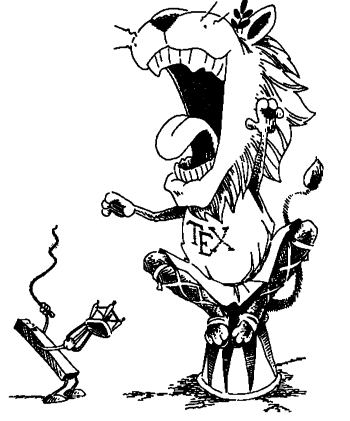
\includegraphics[width = \textwidth]{Chapter3.png}
		\caption{\TeX 的控制系列}\label{subfig:1b}
	\end{subfigure}
	\caption{子图模式测试1:2张图}\label{fig:subfig_test1}
\end{figure}

\begin{figure}[htbp]
	\centering
	\begin{subfigure}[b]{.4\textwidth}
		\centering
		
\includegraphics[width = \textwidth]{Chapter4.png}
		\caption{字体}\label{subfig:2a}
	\end{subfigure}
	\begin{subfigure}[b]{.4\textwidth}
		\centering
		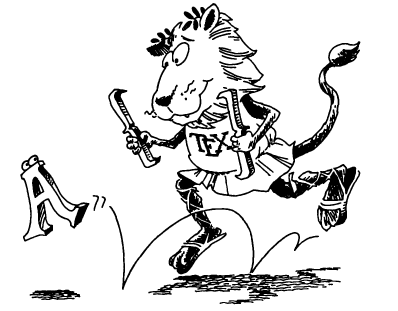
\includegraphics[width = \textwidth]{Chapter5.png}
		\caption{编组}\label{subfig:2b}
	\end{subfigure}
	\begin{subfigure}[b]{.4\textwidth}
		\centering
		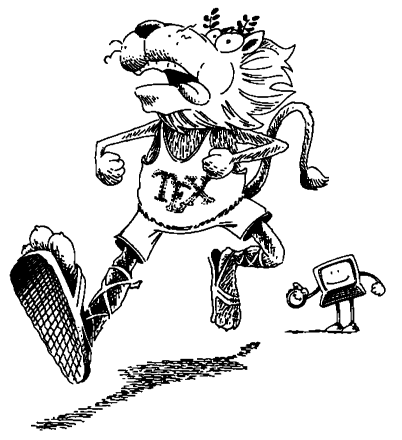
\includegraphics[width = \textwidth]{Chapter6.png}
		\caption{运行\TeX}\label{subfig:2c}
	\end{subfigure}
	\begin{subfigure}[b]{.4\textwidth}
		\centering
		
\includegraphics[width = \textwidth]{Chapter7.png}
		\caption{\TeX 工作原理}\label{subfig:2d}
	\end{subfigure}
	\caption{子图模式测试2:4张图}\label{fig:subfig_test2}
\end{figure}

\subsection{数学模式测试}
数学模式测试,主要测试数学字体,编号和交叉引用。这里首先推荐使用\texttt{align}和\texttt{align*}数学模式环境,大多数行间数学模式只需要用这个环境就可以了。

交叉引用测试,如交引用命令{\ttfamily \textbackslash eqref}和\texttt{\textbackslash ref}命令的区别。如公式\eqref{eq:test1},公式\ref{eq:test1}显示,\texttt{\textbackslash eqref}命令比\texttt{\textbackslash ref}命令的应用结果多了个括号。

如公式\eqref{eq:test3}是单行公式环境,查看公式\eqref{eq:test3}和\eqref{eq:test1}之间的区别,好像在单行公式中没什么区别。
\begin{align}\label{eq:test3}
	f(x) = 2(x + 1)^{2} - 1
\end{align}

\texttt{align}公式环境,用在单行中。
\begin{align}\label{eq:test1}
	f(x) = 2(x + 1)^{2} - 1
\end{align}

\begin{align*}
	f(x) = 2(x + 1)^{2} - 1
\end{align*}
在这里,中间插入一些文字以形成段落,查看行间公式与上下文之间的间隙。下一个公式\eqref{eq:test2}是一个公式组,它在“=”位置对齐。
\begin{align}\label{eq:test2}
	f(x) & = 2(x + 1)^{2} - 1\\
		 & = 2(x^{2} + 2x +1)-1\\
		 & = 2x^{2} + 4x + 1
\end{align}


\section{关于引用}
图表的引用通过{\ttfamily \textbackslash autoref} 命令即可,使用ST LaTeXTools 插件还能自动补全。如果要修改前缀,那么就用{\ttfamily \textbackslash recnewcommand \textbackslash figureautorefname\{好图\}}即可,详见hyperref宏包说明。
